\documentclass[a4paper,10pt]{article}
\linespread{1.0} % Adjust line spacing to avoid font size substitution issues
% \linespread{1.0} % Removed to avoid font size substitution issues
\usepackage[T1]{fontenc} %codifica dei font
\usepackage[utf8]{inputenc} %lettere accentate da tastiera
\usepackage[english]{babel} %lingua del documento
%\usepackage{lipsum} %genera testo fittizio
%\usepackage{tikz}
\usepackage{lmodern}  % Use scalable Latin Modern font
\usepackage{url}
\usepackage{graphicx}
\graphicspath {  { images/ }  }
\usepackage{booktabs}
\usepackage{caption}
\usepackage{subcaption}
\usepackage{hyperref}
%\usepackage{pdfpages}
%\usepackage{rotating}
%\usepackage{tabularx}
%per la tabella
\usepackage{array}
\usepackage{float}  % For the [H] option
\usepackage{xcolor}
\usepackage{colortbl}
%\usepackage{gensymb}
%\usepackage{multirow}
%\usepackage{pdflscape}
%\usepackage{etoolbox}
%\usepackage{color}
%\usepackage{colortbl}
\usepackage{dcolumn}
\usepackage{multirow}
\usepackage{tablefootnote}
\usepackage{amsmath}
\usepackage{listings}
% \usepackage{minted}
\usepackage{amssymb}
\usepackage{makecell}
%\usepackage[margin = 2cm]{geometry} % Almeno abbiamo più spazio
\newcommand{\facciata}
{\newpage\shipout\null\stepcounter{page}}

\usepackage[autostyle,italian=guillemets]{csquotes}

% \usepackage[backend=biber,style=apa,sorting=nyt]{biblatex}
%\usepackage{tocloft}

%\usepackage{titletoc,tocloft}
%\addbibresource{bibliografia.bib}

%\setlength{\cftsubsecindent}{0.5cm}
%\dottedcontents{section}[1.5em]{}{1.3em}{.6em}
%\usepackage{tocloft}

% % Impostazioni per la table of contents
% \setlength{\cftsecindent}{0pt}          % Nessun rientro per le sezioni
% \setlength{\cftsubsecindent}{0.5cm}     % Rientro di 0.5cm per le sottosezioni
% \renewcommand{\cftsecleader}{\cftdotfill{\cftdotsep}}  % Puntini per le sezioni
% \renewcommand{\cftsubsecleader}{\cftdotfill{\cftdotsep}}  % Puntini per le sottosezioni

\usepackage{siunitx}
\usepackage{longtable}

% \title{Data Mining I project: \\
% \textbf{Analyzing Data Insights from the IMDb Platform}}
% \author{Giuseppe Turano, Chiara Ferrara, Alissia Biliotti}
% \date{Academic year 2024/2025}

\usepackage{wrapfig}

\begin{document}

\begin{titlepage}
\setcounter{page}{0} % Imposta il numero di pagina a 0 per questa pagina
\begin{figure}[htp]
\centering

\includegraphics[width=3cm]{cherubino_pant541.pdf} % Logo più piccolo
\end{figure}

\vspace{2cm} % Spazio tra l'immagine e il titolo

\begin{center}
\textbf{\fontsize{18pt}{10pt}\selectfont Data Mining II Project:}\\
\vspace{0.5cm}
\textit{\fontsize{16pt}{10pt}\selectfont Analyzing Data Insights from the IMDb Platform}\\

\vspace{1cm} % Spazio tra il titolo e gli autori
\textbf{Authors:}\\
\vspace{0.3cm}
\text{Bruno Barbieri, Chiara Ferrara, Ankit Kumar Bhagat}



\vspace{10cm} % Spazio tra gli autori e l'anno accademico
\textit{Academic Year 2024/2025}
\end{center}

\end{titlepage}


\tableofcontents

\clearpage


\section*{Introduction}

\section{Data Understanding and Preparation}
The dataset contains 32 columns and 149531 rows of titles of different types.
For each title, the dataset contains information regarding many different
aspects. Table~\ref{tab:initial_categorical_features} lists the initial categorical
features.
\begin{table}[H]
    \centering
    \begin{tabular}{|p{4cm}|p{9cm}|}

        \hline
        \textbf{Feature} & \textbf{Description} \\ \hline
        % Categorical
        \texttt{originalTitle} & Original title, in the original language (?) \\ \hline
        \texttt{isAdult} & Whether or not the title is for adult \\ \hline
        \texttt{canHaveEpisodes} & Whether the title can have episodes \\ \hline
        \texttt{isRatable} & Whether the title can be rated by users \\ \hline
        \texttt{titleType} & Type of the title (e.g., movie, tvseries) \\ \hline
        \texttt{countryOfOrigin} & Countries where the title was primarily produced \\ \hline
        \texttt{genres} & Genres associated with the title \\ \hline
        \texttt{regions} & Regions for this version of the title \\ \hline
        \texttt{soundMixes} & Technical specification of sound mixes \\ \hline
        % Ordinal
        \texttt{worstRating} (ordinal) & Worst title rating \\ \hline
        \texttt{bestRating} (ordinal) & Best title rating \\ \hline
        \texttt{rating} (ordinal) & IMDB title rating class \\ \hline
    \end{tabular}
    \caption{Initial categorical features of the IMDb dataset}
    \label{tab:initial_categorical_features}
\end{table}


Of the initial categorical attributes, the following were removed:
\begin{itemize}
    \item \texttt{originalTitle}, as it did not provide particularly useful
    information;
    \item \texttt{isAdult}, as it was almost completely correlated with the
    \textit{Adult} genre, so a logical OR operation was performed, and the genre
    only was kept;
    \item \texttt{canHaveEpisodes}, as it was completely correlated with the title type
    being \textit{tvSeries} or \textit{tvMiniSeries};
    \item \texttt{isRatable}, as it was always true;
    \item \texttt{soundMixes}, as it required some domain knowledge to be understood, as well as having issues with the values it contained.
    \item \texttt{worstRating} and \texttt{bestRating}, as they were always
    1 and 10, respectively;
    \item \texttt{rating}, as it was obtainable from the \texttt{averageRating}
    continuous attribute, through a simple discretization.
\end{itemize}


Table~\ref{tab:initial_features_numerical} lists the initial numerical features.


\begin{table}[H]
    \centering
    \begin{tabular}{|p{4cm}|p{9cm}|}
        \hline
        \textbf{Feature} & \textbf{Description} \\ \hline
        % Continuous
        \texttt{startYear} & Release year of the title (series start year for TV) \\ \hline
        \texttt{endYear} & TV Series end year \\ \hline
        \texttt{runtimeMinutes} & Primary runtime of the title, in minutes \\ \hline
        \texttt{numVotes} & Number of votes the title has received \\ \hline
        \texttt{numRegions} & Number of regions for this version of the title \\ \hline
        \texttt{totalImages} & Total number of images for the title \\ \hline
        \texttt{totalVideos} & Total number of videos for the title \\ \hline
        \texttt{totalCredits} & Total number of credits for the title \\ \hline
        \texttt{criticReviewsTotal} & Total number of critic reviews \\ \hline
        \texttt{awardWins} & Number of awards the title won \\ \hline
        \texttt{awardNominations} & Number of award nominations excluding wins \\ \hline
        \texttt{ratingCount} & Total number of user ratings submitted \\ \hline
        \texttt{userReviewsTotal} & Total number of user reviews \\ \hline
        \texttt{castNumber} & Total number of cast individuals \\ \hline
        \texttt{CompaniesNumber} & Total number of companies that worked for the title \\ \hline
        \texttt{averageRating} & Weighted average of all user ratings \\ \hline
        \texttt{externalLinks} & Total number of external links on IMDb page \\ \hline
        \texttt{quotesTotal} & Total number of quotes on IMDb page \\ \hline
        \texttt{writerCredits} & Total number of writer credits \\ \hline
        \texttt{directorCredits} & Total number of director credits \\ \hline
    \end{tabular}
    \caption{Initial numerical features of the IMDb dataset}
    \label{tab:initial_features_numerical}
\end{table}

Of the initial numerical attributes, the following were removed:
\begin{itemize}
    \item \texttt{endYear}, as it had no values for non-Series titles, and having around 50\% of missing values for \textit{tvSeries} and
\textit{tvMiniSeries};
    \item \texttt{numVotes}, as it had a very high correlation with \texttt{ratingCount};
\end{itemize}

Figure~\ref{fig:skewness} shows the skewness of some of the numerical features.
It can be observed that many features exhibit a heavy right skew, with a long tail of high values.
Feat
\begin{figure}[H]
    \centering
    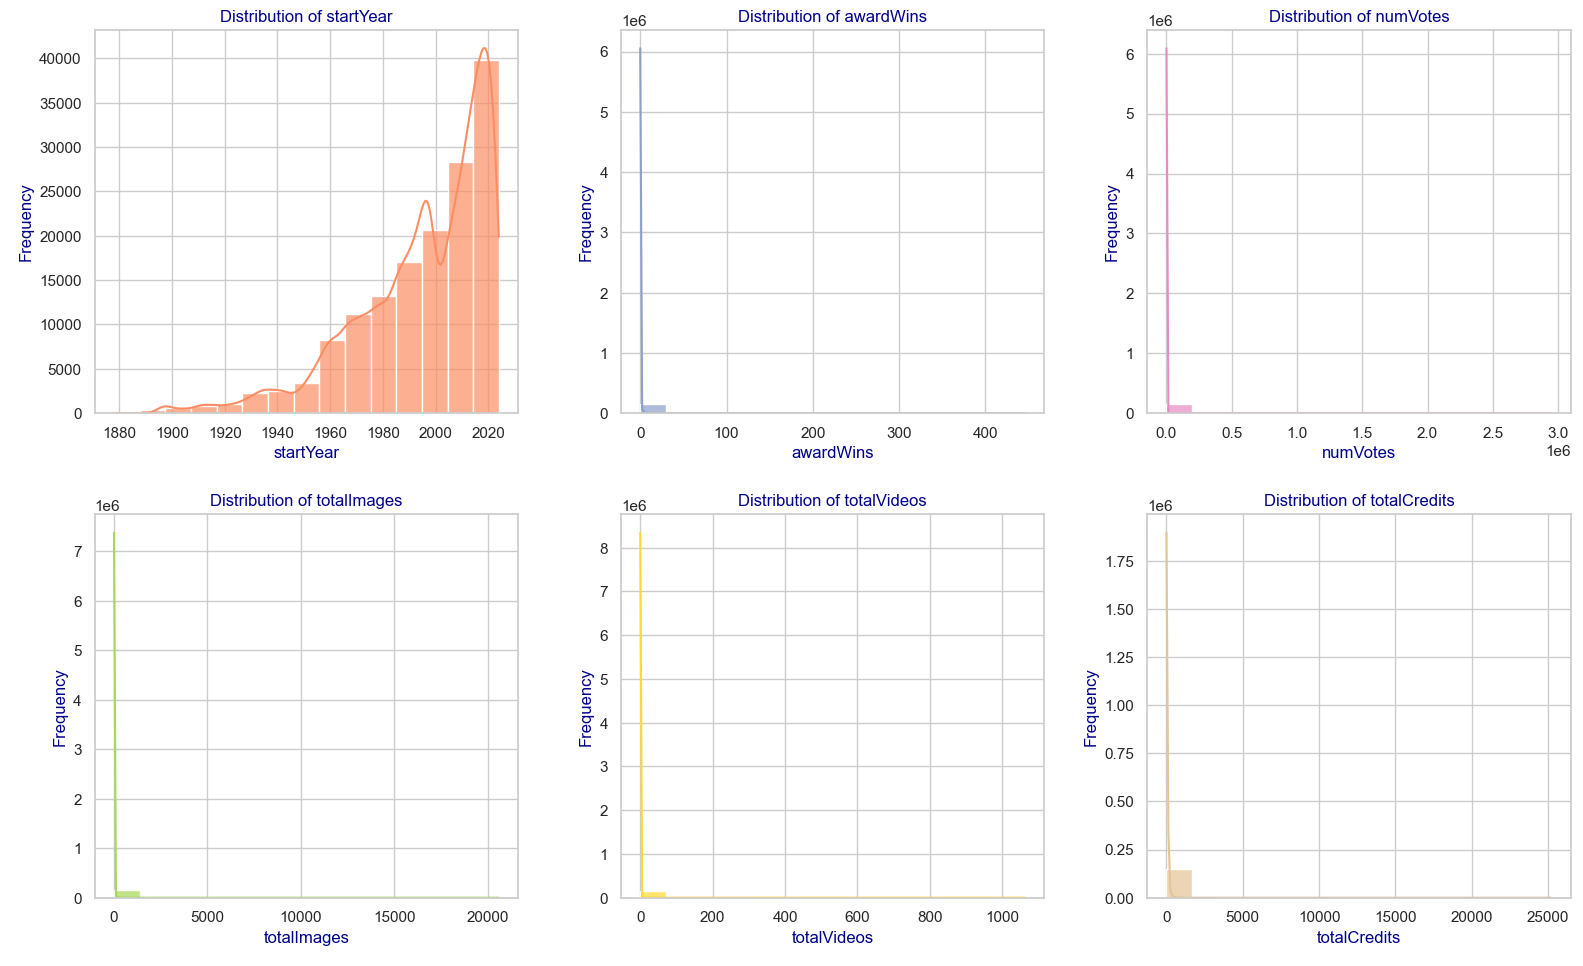
\includegraphics[width=0.6\textwidth]{plotsss/distribution-2.png}
    \caption{Skewness of some numerical features}
    \label{fig:skewness}

Figure~\ref{fig:rating_dist} shows the distribution of the
\texttt{averageRating} attribute.
\begin{figure}[H]
    \centering
    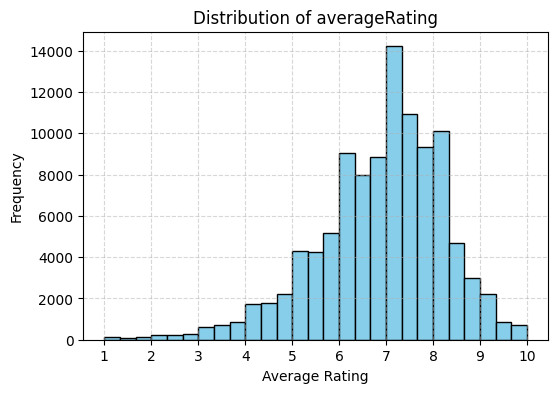
\includegraphics[width=0.6\textwidth]{plotsss/rating_distrib.png}
    \caption{Distribution of the \texttt{averageRating} attribute}
    \label{fig:rating_dist}
\end{figure}
The distribution is Normal-like, with a peak around 7.
This graph is particularly important because of the centrality
of the feature in the classification and regression tasks.



\subsection{Feature Engineering}
\begin{itemize}
    \item \texttt{totalImages}, \texttt{totalVideos} and \texttt{quotesTotal}, were merged
through a simple sum operation
into a single feature (\texttt{totalMedia}) because of their similar semantic
meaning, as well as heavy right skewness;
    \item \texttt{awardWins} and \texttt{awardNominations}, were merged with the same procedure
as above into \texttt{totalNominations}, since they represented the same concept;
    \item \texttt{userReviewsTotal} and\texttt{criticReviewsTotal},were merged with the same procedure
as above into \texttt{reviewsTotal}, since they represented the same concept;
    \item \texttt{regions} and \texttt{countryOfOrigin},
were merged through a simple union operation. The resulting feature was then
represented trhough frequency encoding on the entire list, as well as
counts of the number of countries from each continent.
This resulted in eight new features (six continents, one for unknown country codes,
and the last for the frequency encoding);
    \item \texttt{genre}, it was observed that each record
contained up to three genres, listed in alphabetical order—indicating that the order
did not convey any semantic information about the title.
To represent this information, three separate features were created, each
corresponding to one of the genres. These features were encoded using frequency
encoding, sorted in descending order of frequency across the dataset.  
A value of 0 was used to indicate missing genres—either when no genres were present or
to fill the remaining slots when fewer than three were available;
    \item \texttt{titleType}, was one-hot encoded, as it was a nominal categorical
feature with no intrinsic order;
    \item \texttt{deltaCredits}, was created as the difference between
\texttt{totalCredits} and the sum of \texttt{castNumber}, \texttt{writerCredits} and \texttt{directorCredits}. This feature aimed to capture the number of other types of credits
(such as producers, editors, etc.) associated with a title, which could be relevant for
understanding its production scale and complexity.
    \item \texttt{runtimeMinutes}, had a very high number of missing values approx ~27\%. 
    Since the feature had high relevance in the domain, it was
imputed with the interquartile range, separately for each title
type. For advanced classification, in order to avoid any correlation with the target variable, we imputed the feature with random integers within the global interquartile range.


\end{itemize}



\section{Outliers}
\subsection{Finding Baseline}
In this outlier analysis section, our primary objective was to identify the top outliers in the dataset using three well-established methods- 
\texttt{Local Outlier Factor, Isolation Forest}, and \texttt{Angle-Based Outlier Detection}. 
To establish a baseline for model performance, we initially employed two supervised learning algorithms- 
\texttt{Decision Tree} and \texttt{K-Nearest Neighbors}.
To enhance the alignment between the later module tasks we defined a categorical target variable, \texttt{rating\_bin}, 
by dividing the continuous \texttt{averageRating} into six distinct classes. 
The classes were defined as follows:
\begin{center}
    0 = [0-5); 1 = [5-6); 2 = [6-7); 3 = [7-8); 4 = [8-9); and 5 = [9-10]\\
\end{center}
The value count for each class was 12856, 19576, 37032, 49164, 25414, and 5489 respectively.\\
We then performed a grid search with cross-validation \texttt{(GridSearchCV)} on both models to identify the best hyperparameters. 
Since our dataset was large, we conducted the grid search on a 10\% stratified sample to optimize computational efficiency. 
For K-NN, the optimal parameters were- 
\begin{center}
    metric = 'manhattan', n\_neighbors = 122, weights = 'distance'
\end{center} 
However, to strike a balance between accuracy and computational efficiency, we restricted our model to use \texttt{50 n\_neighbors}. 
For Decision Tree, the optimal parameters were-
\begin{center}
    criterion = 'gini', max\_depth = 10, min\_samples\_leaf = 4, min\_samples\_split = 10, splitter = 'random'
\end{center}
We trained both models on the entire training dataset and evaluated their performance on the test set. 
We split our training dataset into training (80\%) and validation (20\%) sets. We computed the baseline accuracy 
without removing any outliers, which was \texttt{36\% for K-NN} and \texttt{32\% for Decision Tree}.

\subsection{Finding Threshold}
Next, we applied the three outlier detection methods to identify and remove outliers from the training dataset.
We experimented with different contamination levels \texttt{(0.01, 0.05, 0.1)} to 
determine the optimal proportion of outliers to remove.
After removing the identified outliers, we retrained both models on the cleaned training dataset and evaluated their performance on the test set.
We observed that removing outliers generally improved model accuracy, but different contamination levels had no significant impact on the results as shown in table \ref{tab: threshold}.
Only the results from LOF with a contamination level of 0.1 showed an improvement of 1\%. 
Therefore, we fixed the contamination level at 10\% for all three methods to maintain consistency. 
Subsequently, we combined the results of the three methods by aggregating the outlier score and 
removed those rows that were flagged as outliers by at least \texttt{two out of the three methods}, 
which accounted for approximately \texttt{3\%} of the dataset.


\begin{table}[]
\centering
\begin{tabular}{|l|l|l|l|l|}
\hline
 &  & \textbf{LOF} & \textbf{IF} & \textbf{ABOD} \\ \hline
\multirow{2}{*}{\textbf{1\%}} & \textbf{KNN} & 42 & 42 & 41 \\ \cline{2-5} 
 & \textbf{DT} & 39 & 39 & 40 \\ \hline
\multirow{2}{*}{\textbf{5\%}} & \textbf{KNN} & 42 & 42 & 41 \\ \cline{2-5} 
 & \textbf{DT} & 39 & 39 & 40 \\ \hline
\multirow{2}{*}{\textbf{10\%}} & \textbf{KNN} & \textbf{43} & 42 & 41 \\ \cline{2-5} 
 & \textbf{DT} & \textbf{40} & 39 & 40 \\ \hline
\end{tabular}
\caption{Accuracy at different threshold}
\label{tab: threshold}
\end{table}

\subsection{Outlier Detection Conclusion}
In conclusion, our anomaly detection task revealed a consistent trend: both models \texttt{KNN} and \texttt{DT} performed better than the 
baseline after the removal of outliers. This outcome sets the foundation for our subsequent focus on model 
explainability in the later sections.\\ 
From the T-SNE visualization, we observed that \texttt{LOF} predominantly 
identified outliers at the edges of the data distribution \ref{fig:LOF}, whereas \texttt{IF} detected 
them primarily within a clustered region \ref{fig:ISF}. \texttt{ABOD}, on the other hand, captured outliers both at 
the edges and within dense clusters \ref{fig:ABOD}. This variation can be explained by the fundamental 
differences between the algorithms: \texttt{LOF} emphasizes anomalies in low-density regions, 
while \texttt{IF} isolates points distant from the main distribution. 
\texttt{ABOD}, which evaluates outliers based on the angular relationships of points, reflects a hybrid behavior by 
marking anomalies in both sparse and dense regions. Importantly, since the dataset is dominated by a 
single high-density region, most points lack anomalous neighbors, explaining why \texttt{ABOD} highlighted relatively 
fewer strong anomalies. To ensure computational efficiency, we implemented the 'fast' version of \texttt{ABOD}, 
which approximates angle-based detection using a specified number of neighbors rather than exhaustively 
computing angles across all data points. \\
Overall, as we can see from table \ref{tab: threshold} the removal of outliers with different threshold led to only marginal gains in predictive performance.
However, the differences in detection patterns across methods provide valuable insights into the structure and density 
of the data distribution, reinforcing the importance of combining multiple approaches for a more 
comprehensive anomaly detection strategy. Therefore, we combined the results of all three methods to identify the common outliers.


\begin{figure}[htbp]
    \centering
    \begin{subfigure}{0.32\textwidth}
        \centering
        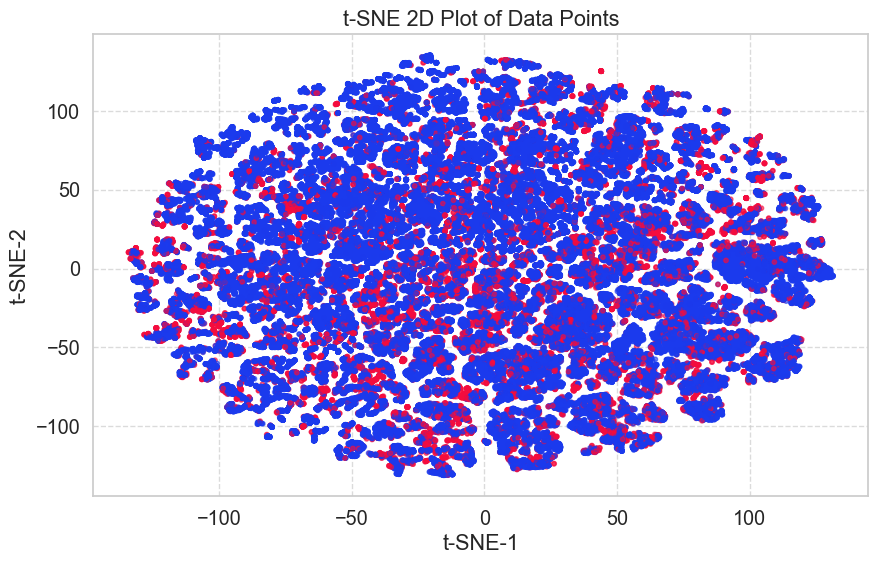
\includegraphics[width=\textwidth]{plotsss/LOF.png}
        \caption{Local Outlier Factor}
        \label{fig:LOF}
    \end{subfigure}
    \hfill
    \begin{subfigure}{0.32\textwidth}
        \centering
        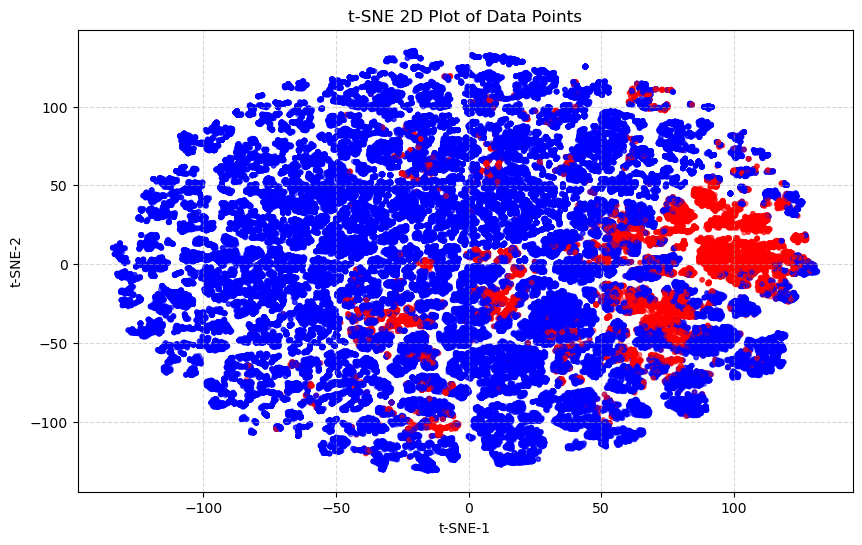
\includegraphics[width=\textwidth]{plotsss/ISF.png}
        \caption{Isolation Forest}
        \label{fig:ISF}
    \end{subfigure}
    \hfill
    \begin{subfigure}{0.32\textwidth}
        \centering
        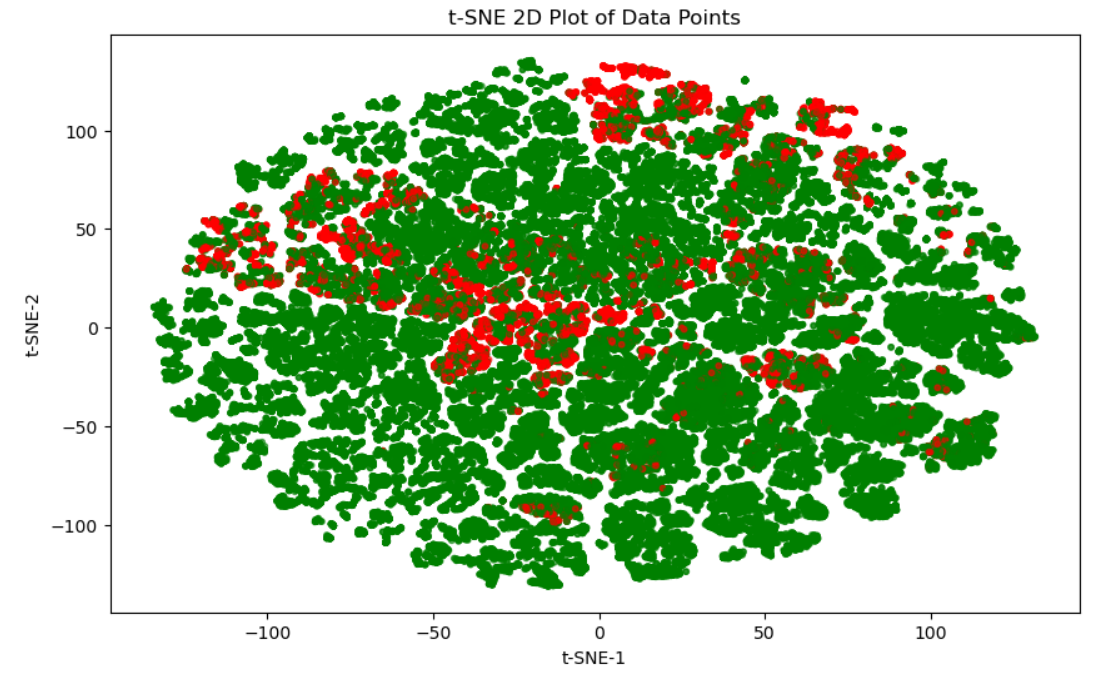
\includegraphics[width=\textwidth]{plotsss/ABOD.png}
        \caption{Angle-Based Outlier Detection}
        \label{fig:ABOD}
    \end{subfigure}
    \caption{Comparison of T-SNE visualizations for different outlier detection methods.}
    \label{fig:outlier_methods}
\end{figure}



\section{Imbalanced Learning}
\subsection{Undersampling}
\subsection{Oversampling}
\subsubsection{SMOTE}


\section{Advanced Classification}
\label{sec:advanced_classification}

In this section, classification results are showcased for two
target variables: \texttt{averageRating} (properly binned into
5 classes), and \texttt{titleType} (with 6 classes).

\textcolor{red}{We then applied multiple classification models using the data as preprocessed previously (see Section~\ref{sec:understanding_preparation}).}   
\textcolor{blue}{The first target variable is \texttt{titleType}, which includes six categories: 
\textit{movie}, \textit{short}, \textit{tvEpisode}, \textit{tvSeries}, 
\textit{tvSpecial}, and \textit{video}. 
The classes are not equally distributed, with \textit{tvSpecial} and \textit{video} 
being significantly under-represented compared to the others. Entries labeled as \textit{videoGame} were removed from both the training and testing sets, 
as they were too few to be useful for classification. 
The remaining categories were merged into broader groups according to the following mapping: 
\textit{movie} and \textit{tvMovie} were grouped as \textit{movie}, 
\textit{short} and \textit{tvShort} were grouped as \textit{short}, 
\textit{tvSeries} and \textit{tvMiniSeries} were grouped as \textit{tvSeries}, 
while \textit{tvEpisode}, \textit{tvSpecial} and \textit{video} were left unchanged. 
All feature columns were standardized using a \textit{StandardScaler}. 
In addition, the variable \texttt{canHaveEpisodes} was removed prior to training, 
since it provides direct information about the target \texttt{titleType} 
and could therefore introduce data leakage.}

\subsection{Support Vector Machines}
\label{subsec:svm}

We applied Support Vector Machines (SVM) to the \texttt{titleType} classification task.
Both linear and non-linear kernels were explored in order to evaluate how decision boundary complexity influences predictive performance.

The first experiment used a Linear SVM trained on the full dataset.  
A grid search with five-fold cross validation was carried out on the parameters 
$C \in \{0.01, 0.1, 1, 10, 100\}$ and $max\_iter \in \{1000, 5000, 10000\}$. 
The optimal configuration, with $C=100$ and $max\_iter=1000$, achieved a test accuracy of 0.81. 
While precision and recall were high for majority classes (\textit{movie}, \textit{short}, \textit{tvEpisode}), 
the classifier failed on \textit{tvSeries}, \textit{tvSpecial}, and \textit{video}, 
indicating that a linear decision boundary is insufficient for this problem.  

Non-linear kernels were then evaluated. 
A grid search was first performed on a stratified 10\% subset of the training set to efficiently explore a wide range of hyperparameters for each kernel, 
since a full search on the complete dataset would have been computationally prohibitive. 
For the RBF kernel, $C$ was varied from 0.01 to 1000 and $\gamma$ between \texttt{scale} and \texttt{auto}. 
The polynomial kernel was tested with $C$ from 0.01 to 100, degree 2--4, $\gamma$ as \texttt{scale} or \texttt{auto}, and \texttt{coef0} 0 or 1. 
The sigmoid kernel was explored over $C$ 0.01--100, $\gamma$ \texttt{scale}/\texttt{auto}, and \texttt{coef0} 0 or 1. 
\textcolor{blue}{Remember to fix C!}

The best configuration for each kernel, reported in Table~\ref{tab:svm_results}, was then retrained on the full dataset and evaluated on the test set. 
Both RBF and polynomial kernels reached approximately 0.90 test accuracy, substantially outperforming the linear baseline and sigmoid. 
The RBF kernel was selected as the reference non-linear model due to slightly more stable results and improved recall on the under-represented classes.


ROC curves were used to evaluate class separability (Figure~\ref{fig:roc_four}),
showing excellent separation for majority classes, although minority categories remained problematic. 

\textcolor{red}{I will change the text and explain the figures better.}

To address class imbalance, the RBF kernel was retrained with \texttt{class\_weight=balanced}, 
which penalizes misclassification of under-represented classes. 
This model reached a slightly lower overall accuracy of 0.84, 
but recall for \textit{tvSpecial} and \textit{video} improved, providing a more equitable classification across categories.  
Confusion matrices (Figure~\ref{fig:rbf_balanced_two}) 
illustrate that \textit{tvSpecial} and \textit{video} ...  
Analysis of the support vectors confirmed this effect. 
In the unbalanced RBF, nearly all points of minority classes became support vectors, 
while in the balanced model the total number of support vectors increased and was more evenly distributed across classes, 
indicating a more complex but fairer decision function. 

Table~\ref{tab:svm_results} summarizes the main results, including the parameters used for each kernel and the corresponding test performance. 


\begin{table}[h]
\centering
\caption{Comparison of SVM models on the IMDb classification task.}
\label{tab:svm_results}
\begin{tabular}{lccc}
\hline
\textbf{Model} & \textbf{Best Params (main)} & \textbf{Test Accuracy} & \textbf{Macro F1-score} \\
\hline
Linear SVM & $C=100$, $max\_iter=1000$ & 0.81 & 0.45 \\
RBF kernel & $C=10$, $\gamma=\text{scale}$ & 0.90 & 0.64 \\
Polynomial kernel & $C=10$, degree=3, $\gamma=\text{auto}$ & 0.90 & 0.64 \\
Sigmoid kernel & $C=0.1$, $\gamma=\text{auto}$ & 0.65 & 0.36 \\
RBF (balanced) & $C=10$, $\gamma=\text{scale}$, balanced & 0.84 & 0.65 \\
\hline
\end{tabular}
\end{table}
    
% --- First figure: four ROC curves side by side ---
\begin{figure}[h]
    \centering
    \begin{subfigure}[b]{0.24\textwidth}
        \centering
        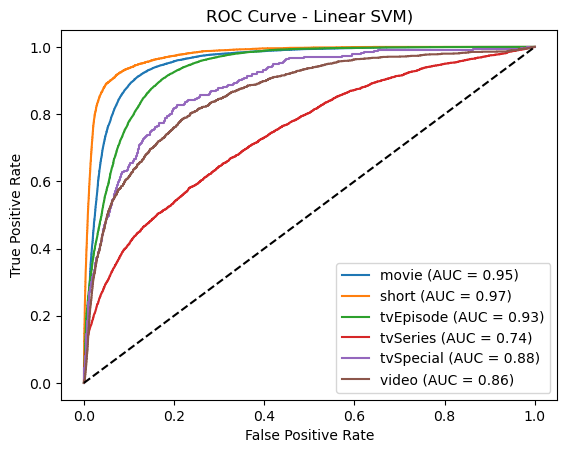
\includegraphics[width=\textwidth]{plotsss/roc_linear.png}
        \caption{Linear SVM}
        \label{fig:roc_linear}
    \end{subfigure}
    \begin{subfigure}[b]{0.24\textwidth}
        \centering
        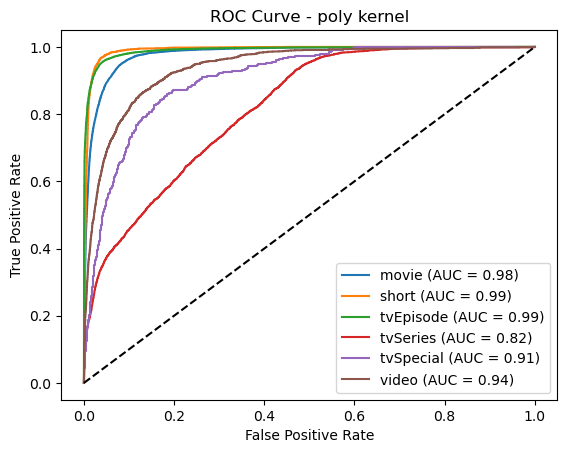
\includegraphics[width=\textwidth]{plotsss/roc_poly.png}
        \caption{Polynomial kernel}
        \label{fig:roc_poly}
    \end{subfigure}
    \begin{subfigure}[b]{0.24\textwidth}
        \centering
        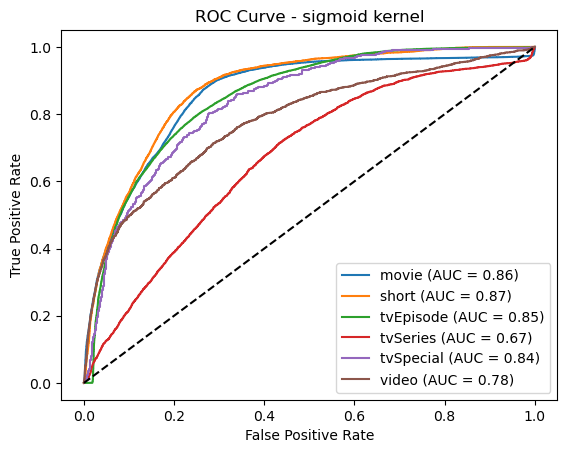
\includegraphics[width=\textwidth]{plotsss/roc_sigmoid.png}
        \caption{Sigmoid kernel}
        \label{fig:roc_sigmoid}
    \end{subfigure}
    \begin{subfigure}[b]{0.24\textwidth}
        \centering
        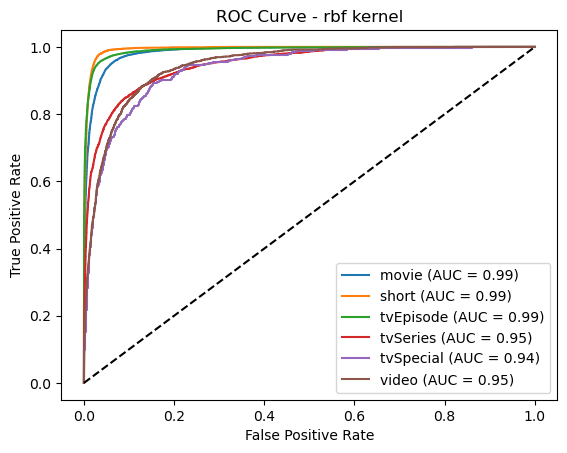
\includegraphics[width=\textwidth]{plotsss/roc_rbf.png}
        \caption{RBF kernel}
        \label{fig:roc_rbf}
    \end{subfigure}
    \caption{...}  
    \label{fig:roc_four}
\end{figure}

% --- Second figure: confusion matrix and ROC for RBF balanced ---
\begin{figure}[h]
    \centering
    \begin{subfigure}[b]{0.48\textwidth}
        \centering
        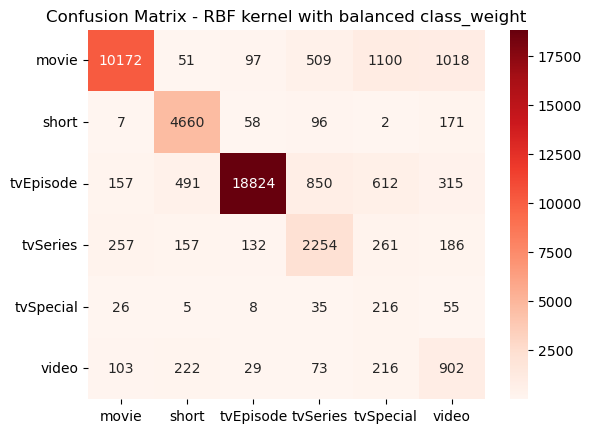
\includegraphics[width=\textwidth]{plotsss/cm_rbf_balanced.png}
        \caption{Confusion Matrix RBF balanced}
        \label{fig:cm_rbf_balanced}
    \end{subfigure}
    \begin{subfigure}[b]{0.48\textwidth}
        \centering
        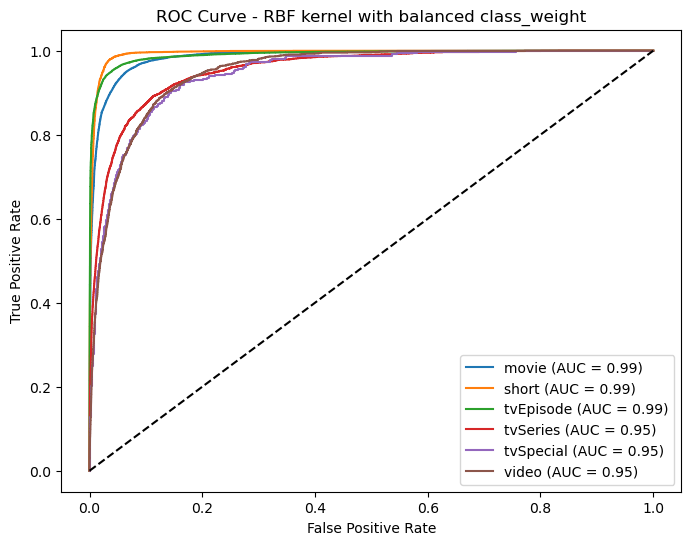
\includegraphics[width=\textwidth]{plotsss/roc_rbf_balanced.png}
        \caption{ROC RBF balanced}
        \label{fig:roc_rbf_balanced}
    \end{subfigure}
    \caption{...}  
    \label{fig:rbf_balanced_two}
\end{figure}

% In conclusion, non-linear kernels were clearly superior to the linear SVM, 
% with RBF and polynomial achieving comparable accuracy. 
% The RBF kernel with balanced class weights provided the best compromise, 
% maintaining strong performance on majority classes while improving recognition of minority ones.

\subsection{Rating classification}
A binned rating classification task was chosen because of how meaningful
the feature is.
Since the feature is continuous, containing float values between 1 and 10,
it was binned in 5 classes:

\begin{itemize}
    \item 0: [1.0, 6.0), containing all insufficient ratings; this class
    represented 
    \item 1: [6.0, 7.0)
    \item 2: [7.0, 8.0)
    \item 3: [8.0, 9.0)
    \item 4: [9.0, 10.0]
\end{itemize}

\subsubsection{Ensemble methods}

\subsubsection{Neural Networks}

\subsection{Title type classification}

\subsubsection{Ensemble methods}

\subsubsection{Neural Networks}

\section{Advanced Regression}

The chosen target variable is \texttt{averageRating}, which represents 
the average rating (on a 1--10 scale) assigned by IMDb users to each title. The exploratory 
data analysis showed that its distribution is approximately normal, 
with most titles concentrated in the range between 6 and 7. 
%For consistency with the classification task, the dataset was split into training 
%(70\%) and test (30\%) sets using the same stratification strategy.

\subsection{Random Forest Regression}
We applied the \textit{Random Forest Regression} algorithm on the task.
Before training the model, although not strictly necessary for tree-based models, 
we standardized the numerical features for consistency and transformed the categorical feature
\texttt{titleType} using \textit{One-Hot Encoding}.

The hyperparameters were optimized using \textit{RandomizedSearchCV} with 5-fold cross-validation, 
exploring different values for the number of trees (100, \textbf{200}, 300, 400, 500), 
the maximum depth (\textbf{None}, 10, 15, 20, 25, 30), 
the minimum number of samples required for a split (2, \textbf{5}, 10, 15) and for a leaf
(\textbf{1}, 2, 4, 6), and the number of features considered at each split (sqrt, \textbf{log2}). 
The best hyperparameters found are highlighted in bold. 
The \texttt{R\textsuperscript{2}} score was used as the evaluation metric during cross-validation.

 
The optimized Random Forest was first evaluated on the test set (results reported in Table~\ref{tab:rf_metrics}).
Subsequently, the model was retrained using only the 18 most important features identified through feature importance analysis.
Feature selection was guided by a cumulative importance plot, which showed that these 18 features accounted for over 90\% 
of the total importance, effectively reducing the dimensionality from the original 28 features without a significant loss in predictive performance.

\begin{table}[h]
\centering
\caption{Performance of the Random Forest Regressor on the test set 
(full model vs reduced features).}
\label{tab:rf_metrics}
\begin{tabular}{lccc}
\hline
\textbf{Model} & \textbf{MAE} & \textbf{MSE} & \textbf{R\textsuperscript{2}} \\
\hline
Random Forest (All Features) & 0.7536 & 1.0833 & 0.4033 \\
Random Forest (Top 18 Features) & 0.7550 & 1.0922 & 0.3984 \\
\hline
\end{tabular}
\end{table}

The results, reported in Table~\ref{tab:rf_metrics}, indicate that the Random Forest model achieves 
a mean absolute error below one point on the IMDb scale and explains around 40\% of the variance in the target variable. 
Notably, the model trained on only the top 18 features performs almost identically to the full-feature model 
(R\textsuperscript{2}: 0.3984 vs 0.4033), showing that 
predictive power is concentrated in a limited subset of variables. 
%These results represent solid performance, especially considering the subjective nature of ratings and the complexity of the domain.

Feature importance analysis further highlighted that the most influential predictors include both numerical variables,
such as \texttt{runtimeMinutes}, \texttt{startYear}, \texttt{ratingCount}, and \texttt{deltacredits},
and categorical variables derived from the encoding step, such as \texttt{titleType\_tvEpisode}, among others. 

\begin{figure}[h]
\centering
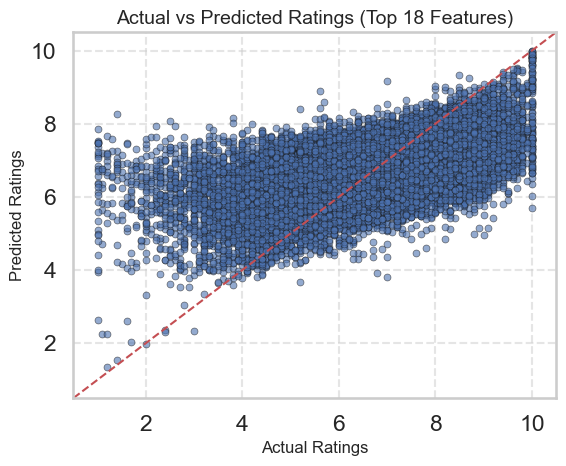
\includegraphics[width=0.7\textwidth]{plotsss/rf_top18_actual_vs_predicted.png} 
\caption{Actual vs Predicted \texttt{averageRating} for the Random Forest model trained on the top 18 features.}
\label{fig:rf_top18_actual_vs_predicted}
\end{figure}


The scatter plot in Figure~\ref{fig:rf_top18_actual_vs_predicted} shows that the predicted ratings roughly follow the trend of 
the actual ratings. Most predictions fall in the 6–7 range, consistent with the distribution of the target variable. 
While the model captures the general pattern, deviations occur, particularly at the extremes, which is consistent with the moderate R² of around 0.40. 
This indicates that the model explains a substantial portion of the variance, but there remains considerable unexplained variability.

% Questione cross validation ???

\subsection{Neural Network Regression}
A feedforward neural network was also implemented for the regression task.

Table~\ref{tab:nn_metrics} summarizes the performance of the neural network on the test set.
\begin{table}[h]
    \centering
    \begin{tabular}{lcc}
        \hline
        \textbf{MAE} & \textbf{MSE} & \textbf{R\textsuperscript{2}} \\
        \hline
        0.7463 & 1.0791 & 0.4067 \\
        \hline
    \end{tabular}
    \caption{Performance of the Neural Network Regressor on the test set.}
    \label{tab:nn_metrics}
\end{table}


\end{document}

